\section{Notation Metamodel} \label{chp:NotMM}
In order to bridge the gap between a model and a token stream, a notation model is developed. The notation model is an EMF model, so it is possible to persist the notation model separately from the language model. The existence of a notation model is optional, after a token stream or a language model is created with one exception. The exception is that the use of morphemes is without default or language element representations. Due to this fact, they should be avoided. It is possible to create a notation model from a word of a language or from a model which complies to the additional constraints introduced by a grammar. The presented notation model does not include additional layout information, for example newlines, spaces, tabs or for visual editor's coordinates, styles, etc. In general, the notation model saves information which is not stored in the language model but relevant for presentation.\\

The main purpose of the notation model is to unambiguously describe a word which produces the language model and to enable a choice of different representations for grammar parts by providing hints for the Guided Parse Tree Constructor.

The main design considerations for the development of the notation metamodel are:
\begin{itemize}
	\item To be able to fully represent and substitute a parse tree, so token creation could be done easily.
	\item To support the creation of the parse tree from an AST. This means that it must be possible to guide the Parse Tree construction process by hints and hold alternative choices to choose. To be able to distinguish alternative productions that require granularity which is close to the one for parse trees.
	\item To have one notation element container per \code{EObject}. This does not only ease reasoning, but also allows stable paths if the corresponding notation element is a generic container. With the use of an \code{ECrossReferenceAdapter} for the referred language model's resource, it is possible to obtain the corresponding notation element even if the structure of the notation model is lost. 
\end{itemize}

Requirements:
\begin{itemize}
	\item In contrast to Xtexts node model which is just updated during parsing and used to guide parse tree construction, the Notation metamodel must be equivalent to a valid token stream and therefore describe it unambiguously. 
	\item It must contain or refer to all information necessary to create a specific token stream together with a language model and a grammar model.   
	\item it has to be a parse tree in order to create language elements if the corresponding tokens exist.
	\item it should offer GMF stuff elements \todo{add what GMF has interesting}
	explicitly separated from language model
\end{itemize}

A notation model will refer grammar elements, so before the notation metamodel can be developed, an EBNF grammar metamodel will be defined.

As convention, transient model elements are modeled as private static elements, thus with a leading \code{-} and are \underline{underlined}.


\subsection{Notation Metamodel}
\todo{rename topic}
%% Prod
\begin{figure}
\centering
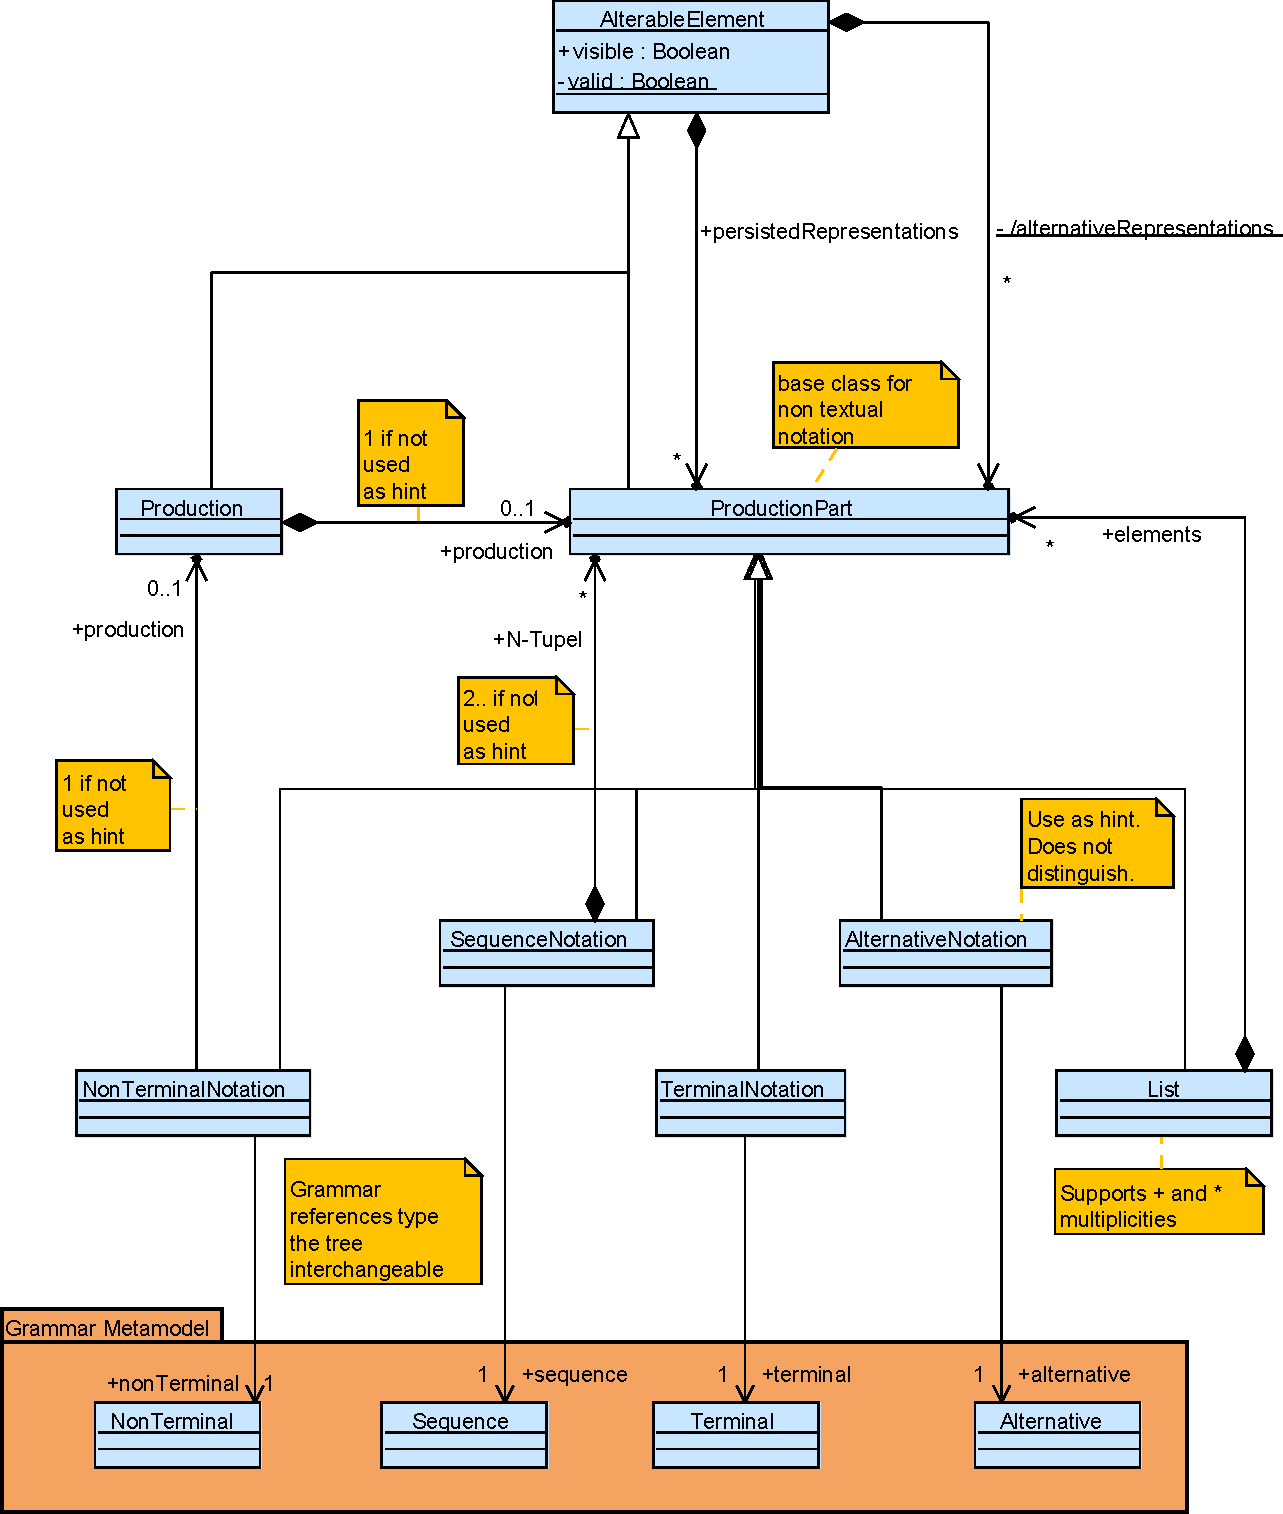
\includegraphics[scale=0.65]{gfx/ex/Notation_Prod} 
\caption{Production part of Notation metamodels}
\label{MM:Not:Prod}
\end{figure}

The diagram \ref{MM:Not:Prod} shows the section of the notation metamodel which is relevant for its function representing a parse tree and guiding Parse Tree construction. It is able to represent parse trees up to terminals, but does not contain the token values.\\

\subsection{Evolving from a simple parse tree metamodel} The metamodel in diagram \ref{MM:Not:PT} is sufficient to describe a parse tree, where \code{TerminalNotation}s represent the leafs and \code{NonTerminalNotation} the branches. It contains a subset of elements of the notation model, namely \code{NonTerminalNotation}, \code{TerminalNotation} and \code{ProductionPart}. The relationship of the subset elements differs from \ref{MM:Not:Prod} in that \code{NonTerminalNotation} contains \code{ProductionPart}s directly, but more importantly also that \code{NonTerminalNotation} can contain multiple \code{ProductionPart}s. \code{NonTerminalNotation} and \code{TerminalNotation} are of a generic type, to determine which Symbol they represent, they refer to \code{NonTerminal} and \code{Terminal}. The distance\footnote{\raggedright between nodes in a graph} to the symbol is one, the distance to the symbol type is two. 
For example, in the following grammar, the type of the \code{b}s are equal, but the \code{b}s are not:\\
\code{S : b c | b d} \\
A verbose representation of this grammar would be: \\
\code{S : b$_1$ c | b$_2$ d} \\
The \code{TerminalNotation}s refer to the exact position in the grammar, regarding the previous case for example to \code{b$_1$}, which refers itself to the type \code{b}. For an concrete parser implementation, this means that in case of a shift reduce parser, the reference to the \code{NonTerminal} can be at least one production later than normal, because the type is known when the rule is reduced, but the position is not known until its producing production is reduced. The exact positions are useful to guide Parse Tree construction and the referencing solution provides flexibility while keeping stable \code{NonTerminalNotation}s and \code{TerminalNotatation}s. The parse trees that are created by this metamodel need post processing to group their structure. \\
For example, accessing the last \code{b} in the tree created by the grammar for the input \code{b b b c b} requires an iteration over each element:\\
\begin{xtxt}
A : b+ c b 
\end{xtxt}


\begin{figure}
\centering
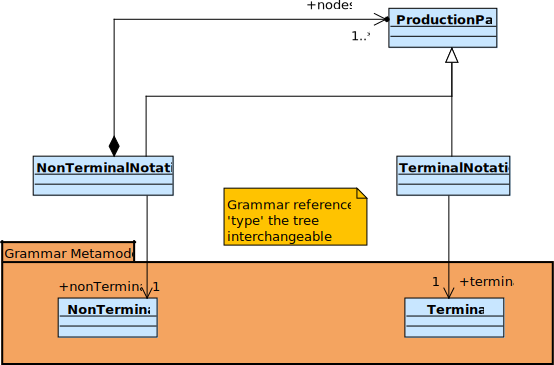
\includegraphics[scale=0.75]{gfx/ex/Notation_ParseTree} 
\caption{Simple parse tree metamodel}
\label{MM:Not:PT}
\end{figure}

\subsection{Term parse tree metamodel} A metamodel able to hold terms structured is shown in \ref{MM:Not:TT}. The \code{NonTerminalNotation} holds exactly one reference to a \code{ProductionPart} named \code{production}. The distinction in different terms is held by \code{SequenceNotation} which contains an \code{n-tuple} of at least two \code{ProductionPart}s. A \code{List} holds \code{Symbol}s with a possible multiplicity higher than one. It might be beneficial to directly support multiple values per \code{ProductionPart}, for example \code{a+}, but this would not render \code{List} obsolete in order to support \code{(a | B)+}. Since alternatives do not occur in a parse tree, because one choice must have been used, they have no equivalent in the term parse tree metamodel. 

\begin{figure}
\centering
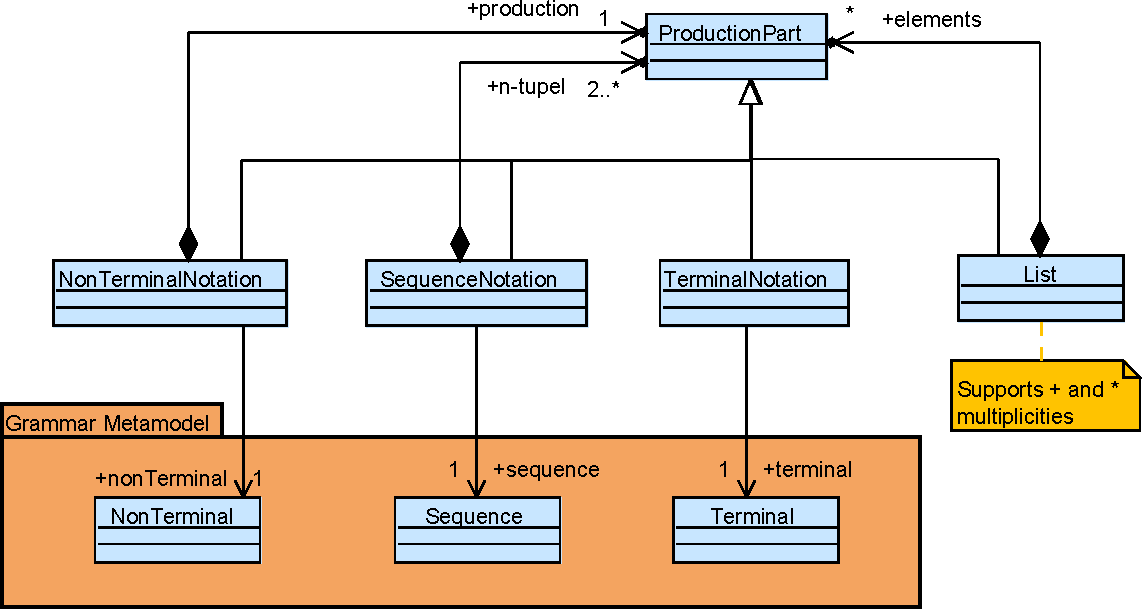
\includegraphics[scale=0.75]{gfx/ex/Notation_TermTree} 
\caption{Term parse tree metamodel}
\label{MM:Not:TT}
\end{figure}

\subsection{Production part of the Notation model}
Figure \ref{MM:Not:Prod} shows the final production part of the notation metamodel. It differs from the one used for terms in the following points:
\begin{itemize}
	\item an additional indirection from \code{NonTerminalNotation} to \code{ProductionPart} was introduced. 
	\item \code{AlternativeNotation} to represent \code{Alternative}s was added.
	\item The multiplicities of the references are less constrained regarding the lower bound.
	\item \code{AlterableElement} was added.
\end{itemize}
The use of the additional indirection from \code{NonTerminalNotation} to \code{ProductionPart} via \code{Production} decouples the \code{Production}. The reason for this is the use of \code{Production} as the complementing element for a language element. This is described in more detail in \todo{ref} and is one of the main design targets of the notation model.\\
As stated in \todo{ref} \code{AlternativeNotation} is not needed to represent a parse tree. It is the only \code{ProductionPart} which does not contain and does not refer to data or another \code{ProductionPart}. \code{TerminalNotation}'s link to data is described in the separate diagram \ref{MM:Not:DataLink}. \code{AlternativeNotation}'s only use is to hint while the parse tree is constructed. For example, without \code{ProductionPart} for the given rule
\begin{xtxt}
R : ((a | b) | (c d)) 
\end{xtxt}
it is possible to hint to each element individually, but it would be impossible to hint to the alternative \code{(a | b)}. \\
To be able to hint to a specific grammar element without requiring a representation is the reason the lower bounds of all references have been removed. This must be possible during parse tree construction.\\
\code{AlterableElement} is the base class of all production related classes. Its main task is to hold \code{alternativeRepresentations} for itself. These \code{alternativeRepresentations} are not persisted and are derived by the Parse Tree Constructor or in other words set by it. \code{AlterableElement}s also contains a set of \code{persistedRepresentations} maintained from former representations, for example. These do not need to be a subset of the current \code{alternativeRepresentations}. Its dedicated use is to restore former representations, which are or became again valid.

\subsection{Production part of the Notation model} \label{sec:MM:Not:Prod}
Figure \ref{MM:Not:LR} shows how the connection of the Notation metamodel to the language model is made. The two central metaclasses in this diagram are \code{EObjectProduction} and \code{LanguageTokenContent}. The root of the notation model is \code{NotationModelRoot}. It contains the \code{rootProduction} of the parse tree. This might be an \code{UnassignedRuleProduction}, but in general an \code{EObjectProduction}. The connection between both is established by the reference \code{languageElement} of \code{EObjectProduction}.  The type of the referred instance must be the referred type of the \code{EObjectTypeRule} at \code{type} references of \code{EObjectProduction}. \code{EObjectProduction}s are the only notation elements which establish a direct connection between the notation model and the language model. \code{EObject}s, like Java objects, are the only referable instance at runtime. Thus, a structurally identical containment relationship based tree with language objects on the one hand and \code{EObjectProduction}s are created on the other side. The subtrees of a notation node, \code{EObjectProduction}, are stored in its \code{children} containment. This complements the vanished containment relation between \code{NonTerminalNotation} and \code{Production} in figure \ref{MM:Not:PT}. This design allows each \code{EObject} production to contain its own part of the parse tree, integrating parse tree and structurally symmetric language tree on a per \code{NonTerminalNotation} base. \code{NonTerminal}s are the only part in the grammar where \code{EObject}s are produced, but \code{NonTerminal}s may also produce \code{EDataType}s or refer to a rule which is an unassigned rule call. To store productions in the parse tree where no \code{EObject} is produced, \code{NonTerminalNotation} contains a derived \code{nonEObjectProduction} containment. This containment is derived, because it is just set in the case where \code{production} is not of type \code{EObjectProduction}. This reestablishes the missing containment reference in the case where the \code{Production} is not contained by the \code{EObjectProduction} tree. \\
The other notation class, which needs to establish a connection to the language elements, is \code{LanguageTokenContent}. The \code{TokenContentAdapter} is responsible to fill in the token value while the token stream is created during token stream creation of the parse tree. This is explained in \todo{ref}. \code{LanguageTokenContent} is responsible to assign the token content based on a value of an instance of an \code{EStructrualFeature} of an \code{EObject} in the language model. Because instances of \code{EStructuralFeature}s are not referable, \code{LanguageTokenContent} uses a reference to the \code{EObject} and reflection to obtain the value of the \code{EStructuralFeature} instance defined by the \code{eStructuralFeature} reference of \code{FeatureOperation} of the attributed grammar metamodel. The reference to the necessary language \code{EObject} is obtained by the first parent \code{EObjectProduction} in the notation models containment hierarchy. The \code{index} of \code{LanguageTokenContent} determines the exact value of an \code{eStructuralFeature} in case of a multiplicity higher than one, for example, if an \code{EAttribute} is the type of multiple (list of) strings. 

%% Prod
\begin{figure}
\centering
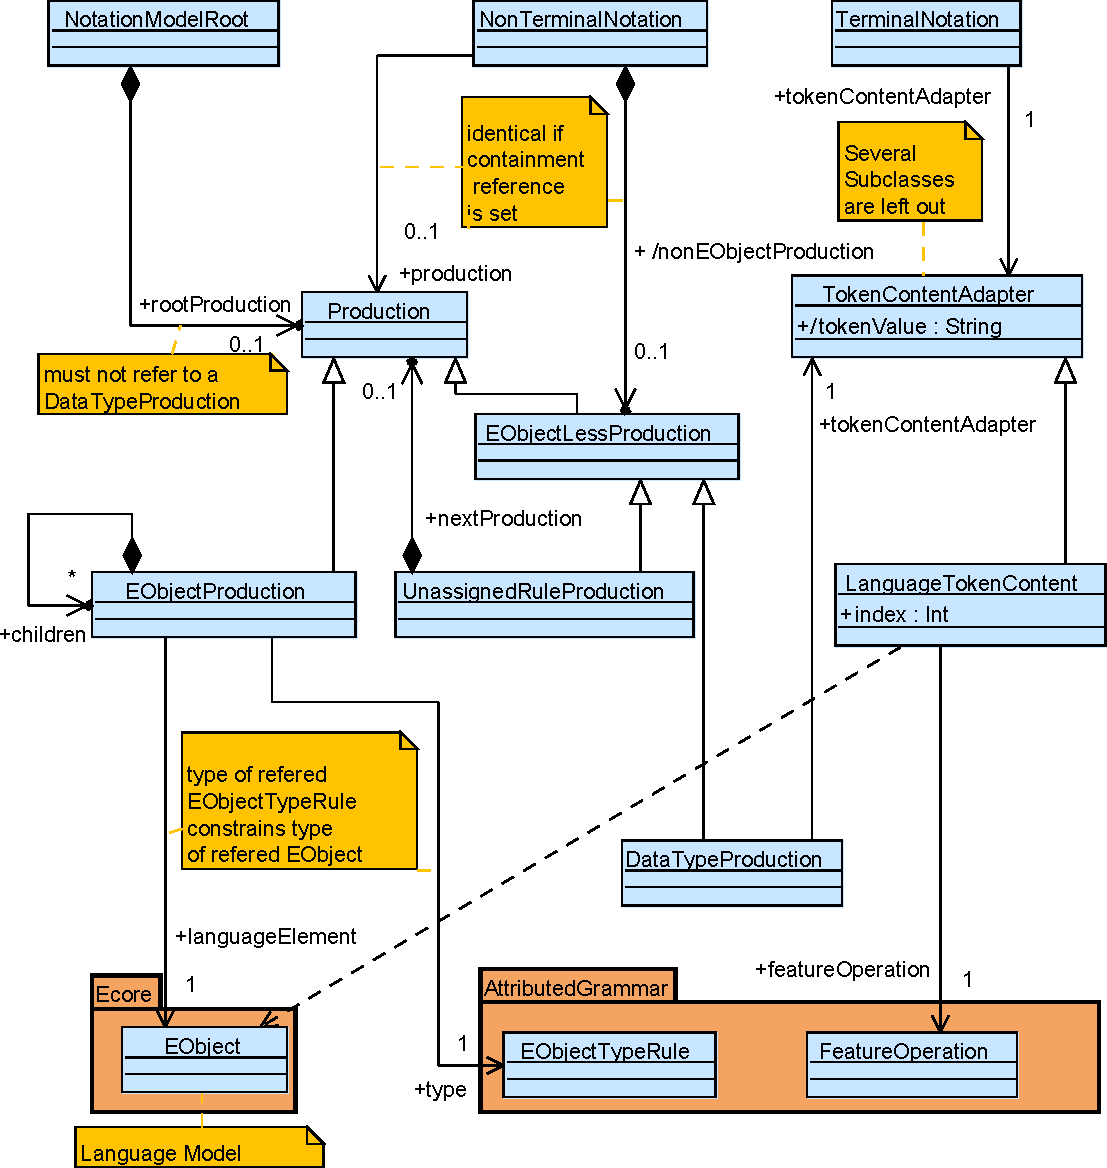
\includegraphics[scale=0.8]{gfx/ex/Notation_LangRel} 
\caption{Language model connection}
\label{MM:Not:LR}
\end{figure}

\subsection{Token value connection}
Diagram \ref{MM:Not:DataLink} shows the relation of notation elements to the token value. Except for the \code{token} reference of \code{TokenContentAdapter}s, this is only relevant for token stream creation of the parse tree. The abstract \code{TokenContentAdapter} is the central class in the diagram. Each \code{TerminalNotation} and each \code{DataTypeProduction} refers to exactly one \code{TokenContentAdapter}. Because both hold the content of a structureless value, this unifies both in regard to token stream creation. The \code{TokenContentAdapter} has a derived attribute named \code{tokenValue} of type string. The value of \code{tokenValue} is determined by the use of \code{ValueConverter}s, in order to convert between a non-character type, for example \code{EInteger} and the only valid output value of Tokens, characters. The use of the transient optional reference to \code{Token} is twofold, first it enables the Notation model to hold references to both, the content of a \code{Token} on the token stream and its content in the language model, thus optionally keeping both synchronized. Second, this existence is mandatory to hold the textual representation of cross references until they are resolved to an URI or completely. Subclasses of \code{TokenContentAdapter}s represent the different possibilities of data sources for the token content:
\begin{itemize}
	\item \code{LanguageTokenContent} is explained in \ref{sec:MM:Not:Prod}.
	\item \code{GrammarTokenContent} the value of the token depends on a \code{Literal} \code{value} defined in the grammar metamodel.
	\item \code{NotationTokenContent} the value of the token is contained by a \code{NotationProperty} in the notation model. The key is obtained by a reference to an instance of \code{NotationPersistedElement}s from the attributed grammar metamodel.
	\item \code{MagicTokenContent} is used when the data source is none of the above. It is used if the content is set programmatically.
\end{itemize}


\begin{figure}
\centering
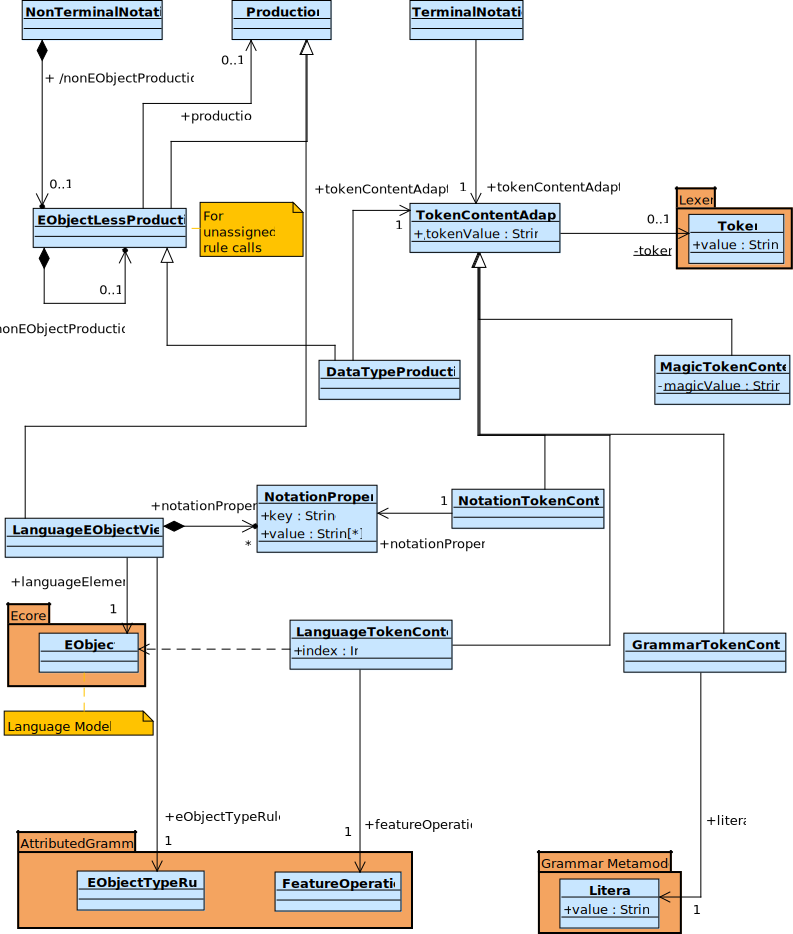
\includegraphics[scale=0.68]{gfx/ex/Notation_DataLink} 
\caption{Token value connection}
\label{MM:Not:DataLink}
\end{figure}

\subsection{Compression of the notation model}
To create a token stream it is necessary to create the complete parse tree structure in the notation model. This structure is more verbose than what is necessary to uniquely identify a word. Due to the fact that the notation model serves as a building plan to create a word, it is just necessary to persist the part of the notation model which eliminates all ambiguities. For example, for the following rule:
\begin{xtxt}
A:  "keyword1" v=ID 
 |  "keyword2" v=ID
\end{xtxt}
it is just necessary to store which rule was chosen, for example, the one containing \code{"keyword1"}, but not the expanded parse tree. If Parse Tree construction is predictable, it is even possible to omit this distinction if the selected option equals the default option of the Parse Tree Constructor.  \\
It is furthermore possible to enumerate the alternatives and save their values instead of the references to the \code{ProductionPart}s.

\subsection{Parse Tree Constructor Conclusion}
The Guided Parse Tree Constructor combined with the notation model allows for the choice of different textual representations for a language model. 



